%%% LaTeX Template
%%% This template is made for project reports
%%%	You may adjust it to your own needs/purposes
%%%
%%% Copyright: http://www.howtotex.com/
%%% Date: March 2011

%%% Preamble
\documentclass[paper=a4, fontsize=11pt]{scrartcl}	% Article class of KOMA-script with 11pt font and a4 format
\usepackage[T1]{fontenc}
\usepackage{fourier}

\usepackage[english]{babel}															% English language/hyphenation
\usepackage[protrusion=true,expansion=true]{microtype}				% Better typography
\usepackage{amsmath,amsfonts,amsthm}										% Math packages
\usepackage[pdftex]{graphicx}														% Enable pdflatex
\usepackage{url}
\usepackage{graphicx}

%%% Custom sectioning (sectsty package)
\usepackage{sectsty}												% Custom sectioning (see below)
\allsectionsfont{\centering \normalfont\scshape}	% Change font of al section commands


%%% Custom headers/footers (fancyhdr package)
\usepackage{fancyhdr}
\pagestyle{fancyplain}
\fancyhead{}														% No page header
\fancyfoot[C]{}													% Empty
\fancyfoot[R]{\thepage}									% Pagenumbering
\renewcommand{\headrulewidth}{0pt}			% Remove header underlines
\renewcommand{\footrulewidth}{0pt}				% Remove footer underlines
\setlength{\headheight}{13.6pt}


%%% Equation and float numbering
\numberwithin{equation}{section}		% Equationnumbering: section.eq#
\numberwithin{figure}{section}			% Figurenumbering: section.fig#
\numberwithin{table}{section}				% Tablenumbering: section.tab#


%%% Maketitle metadata
\newcommand{\horrule}[1]{\rule{\linewidth}{#1}} 	% Horizontal rule

\title{
		%\vspace{-1in} 	
		\usefont{OT1}{bch}{b}{n}
		\normalfont \normalsize \textsc{University of Chicago Dept of Genetic Medicine} \\ [25pt]
		\horrule{0.5pt} \\[0.4cm]
		\huge PGRNseq Analysis \\
		\horrule{2pt} \\[0.5cm]
}
\author{
		\normalfont 								\normalsize
        Vassily Trubetskoy \\[-3pt]		\normalsize
        \today
}
\date{}


%%% Begin document
\begin{document}
\maketitle
\section{Overview}

Report on the analysis of sequence and chip data collected on 253 individuals undergoing chemotherapy with the drug Irinotecan.

\section{Data}

	\subsection{Genotypes}

We currently have access to two different sets of genotypes for this population:
	
	\begin{enumerate}
		\item PGRNseq sequence data on VIP pharmacogenes.
		\item Illumina Exome Chip data. Run as an internal QC measure at the UW.
	\end{enumerate}
	
We have the alignment files for the sequence data. These were run with

	\subsection{Phenotypes}
	
The primary phenotype for this dataset is pharmacokinetic and pharmacodynamic data on patients. These PK/PD models are being generated at the University of North Carolina Chapel Hill.

In addition to PK/PD phenotypes, we are interested in looking at Neutropenia in patients. This is currently coded as the Neutrophil Count Nadir (NCN). This is defined as the lowest Neutrophil count observed in a patient during their course of therapy.

There are several relevant covariates available:
	\begin{itemize}
		\item site of collection
		\item sex
		\item drug dose
		\item self-reported ancestry
	\end{itemize}

	\subsection{Quality Control}
	Consensus calling in the sequence data. The results look very nice for the metrics that we have available (reference separate report, or put figures here).
	
	Exclude rare SNPs in single marker analyses.
	Exclude SNPs out of HWE.
	Exclude SNPs with high rates of genotype missingness.
	Exclude SNPs with low QUAL

	\subsection{Proposed Analyses}
	\begin{itemize}
		\item Linear regression. Using the estimated effect and its eror as a t-statistic. (GenABEL package in R)
		\item SKAT burden test. (SKAT package in R)
	\end{itemize}

\section{Results}

	\subsection{Population Structure}
Sequence data provides too few variants to adequately identify ancestry through PCA .

The Exome chip data \emph{does} provide enough markers to differentiate samples. The spatial axes are well defined.

\begin{figure}
\centering
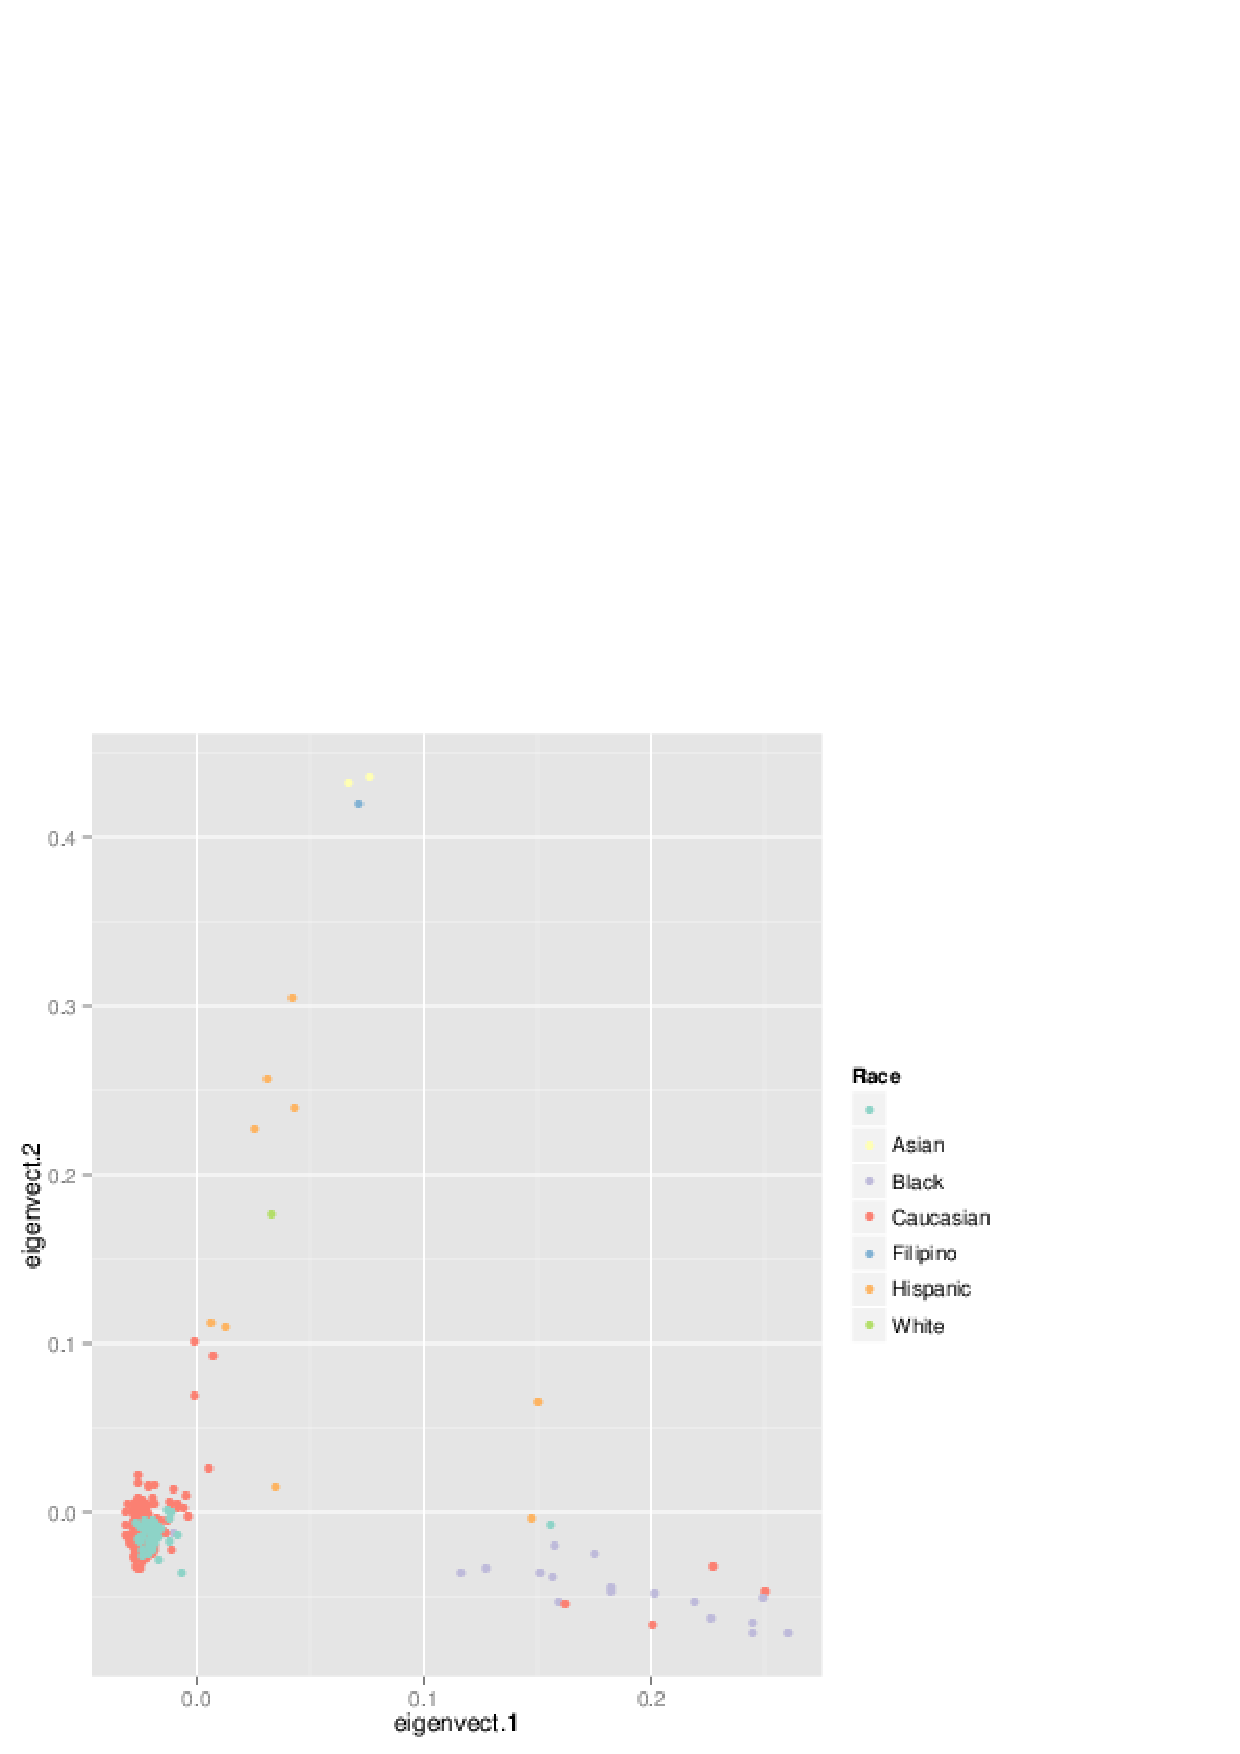
\includegraphics[width=1.0]{plot/exomeChip.PCA.selfReportedAncestry.pdf}
\end{figure}


	\subsection{Single Marker}
		\subsubsection{GenABEL Linear Regression}
		No results in sequence data for common variants.
		One significant results in Exome chip data
		\subsubsection{GenABEL Score Test}
	\subsection{Gene-based}
		\subsubsection{SKAT Burden}
		\subsubsection{SKAT Rare + Common}
		\subsection{Variance Components}

\section{References}


%%% End document
\end{document}
